Different solution for having a multi robot production facility has been discussed among the group. These discussion will be discussed among the other groups in the RSD course. A data flow diagram is shown in figure \ref{fig:ideasForImplementation}. 

\begin{figure}[ht]
\centering
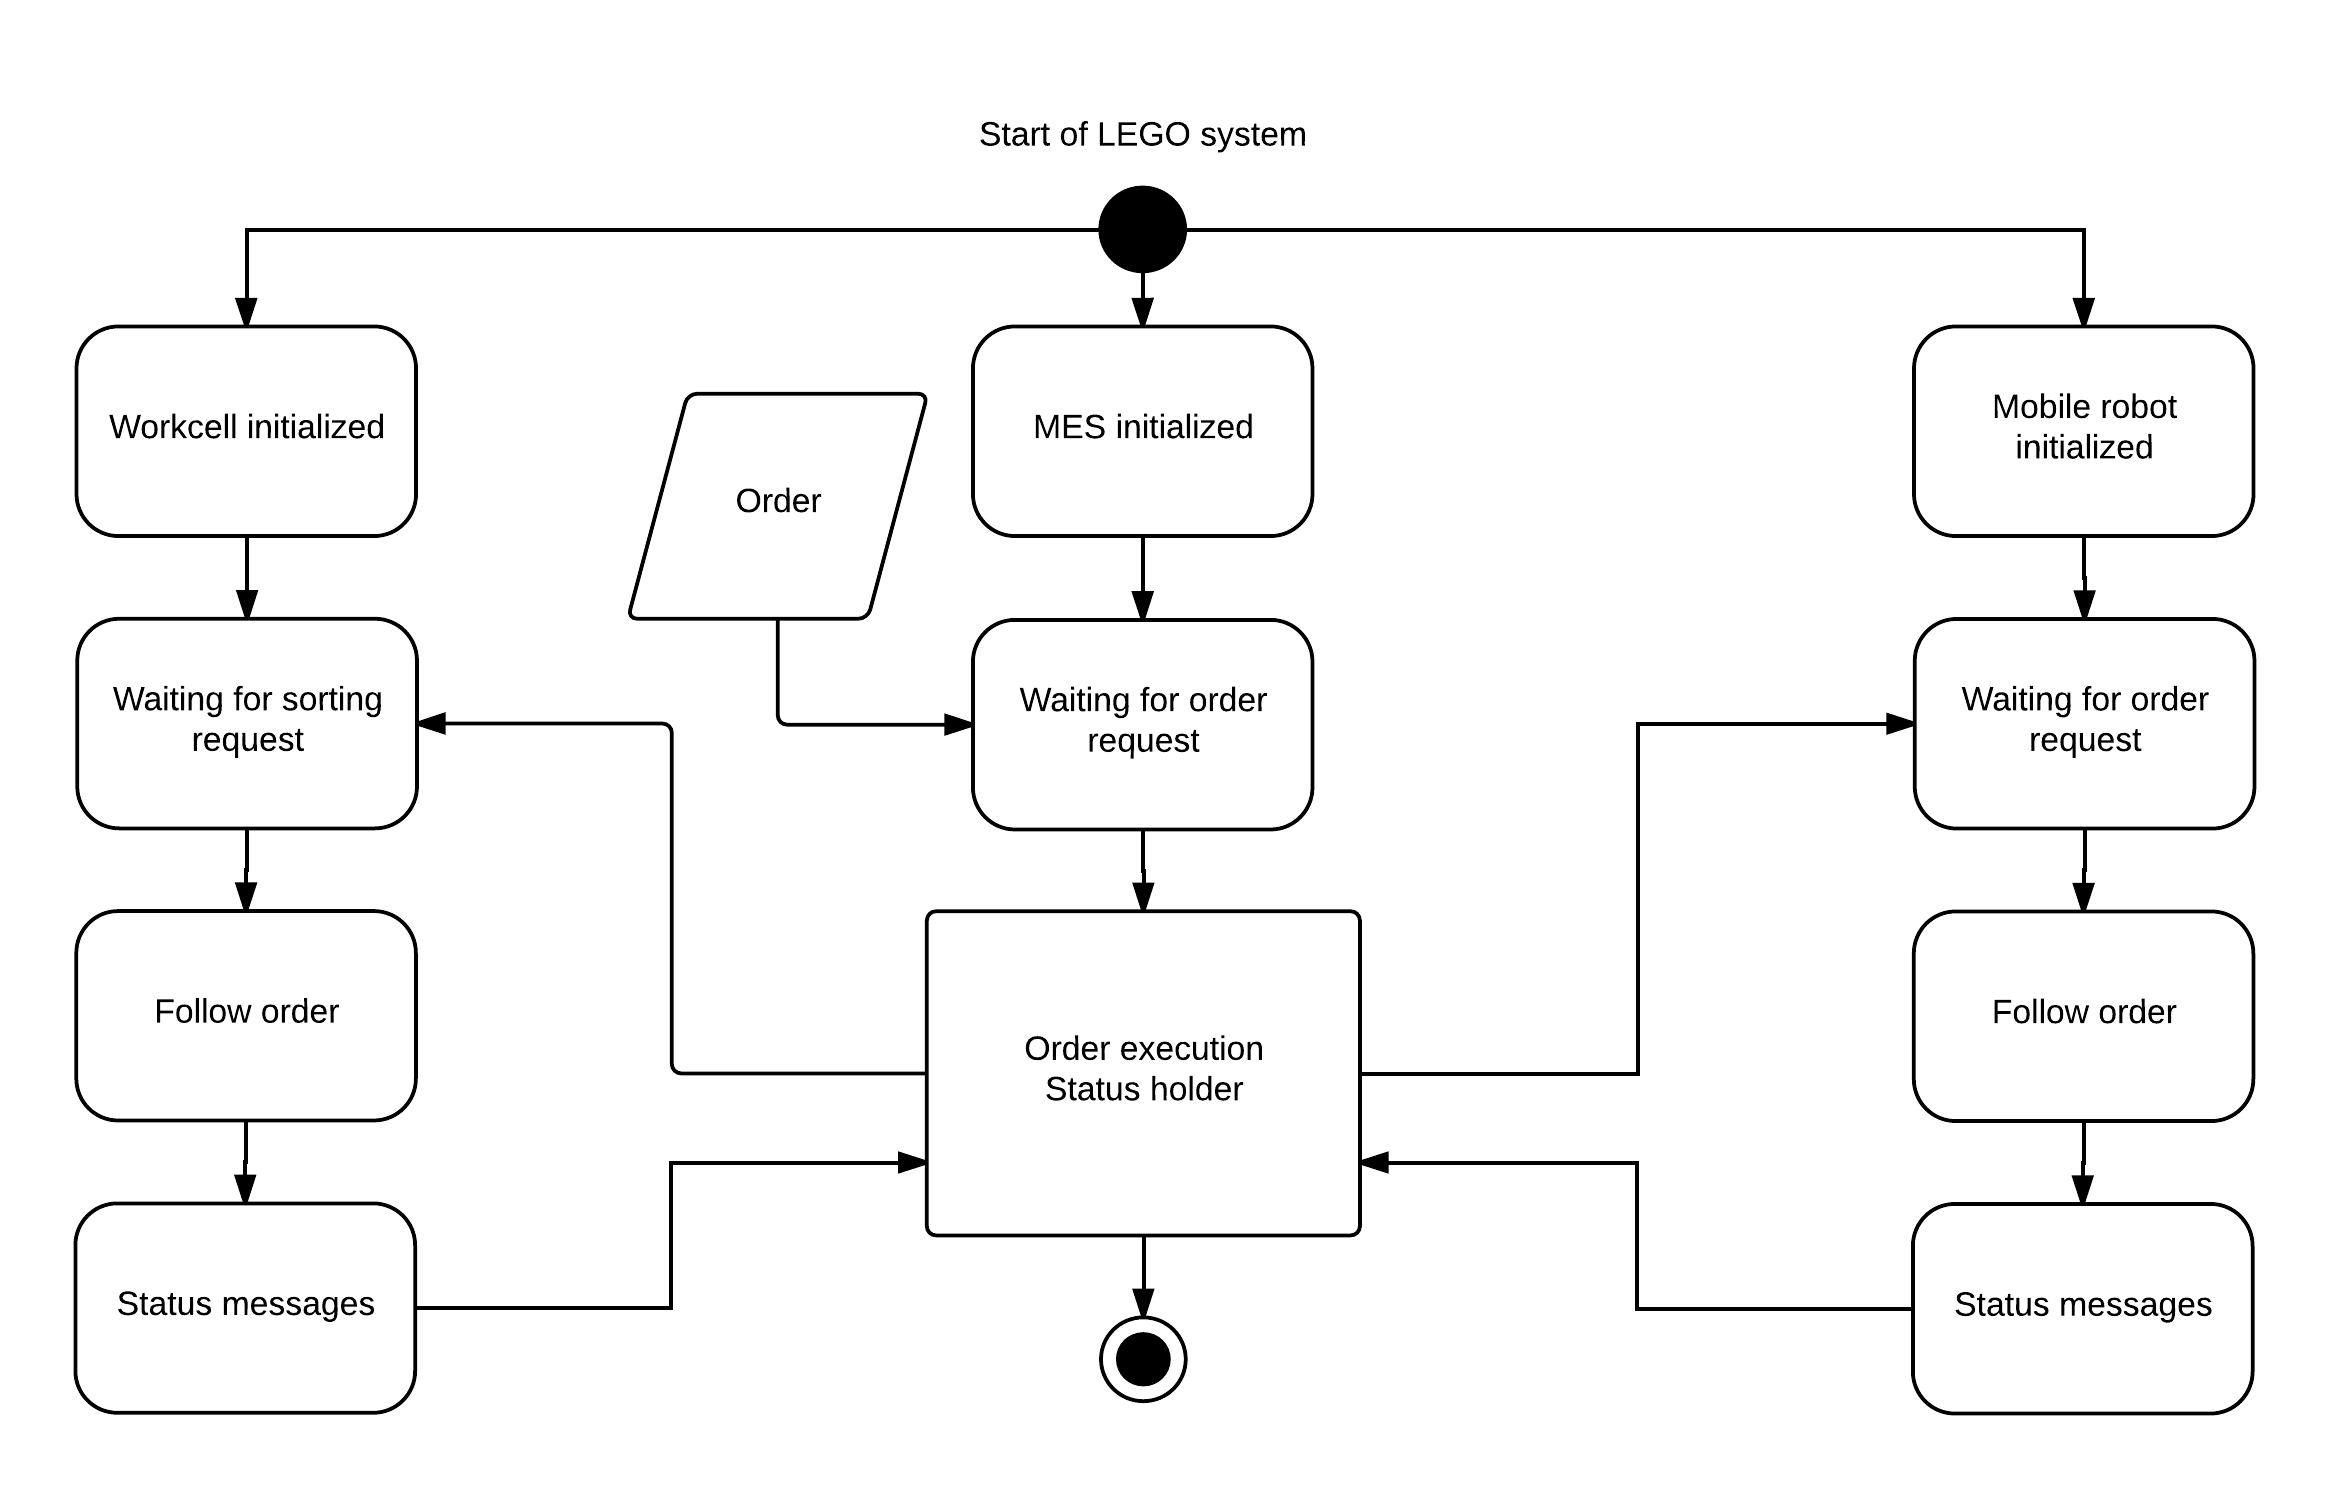
\includegraphics[width=\textwidth]{images/ideasForImplementation.png}
\caption{Idea for flow diagram between MES server, mobile robot and workcell robot}
\label{fig:ideasForImplementation}
\end{figure}

Initially the workcell robot is standing in a initial configuration and the system in the robot cell is waiting for status request or order request from the MES server. If an order is placed in the MES system, an mobile robot will be ordered to pick up bricks from the LEGO dispenser, which feed the mobile robot with a random number of LEGO bricks in a random shape and color. However limitations on the LEGO-bricks will be stated later in the project. 

The MES server will be sending status request for all the robot workcell and receive status if workcells are available or not.
While the mobile robot has been received LEGO-bricks from the dispenser, the MES server has arranged which workcell the current mobile robot has to go to. After the mobile robot acknowledge this order, MES server is sending status report to system in workcell. While mobile robot is under way, the system in workcell gets ready for incomming load-off. The moment the mobile robot get to the barcode, that indicate the target workcell, the mobile robot will send status to the MES server. The MES server will then send loading request to the given workcell, in order begin the loading and sorting of LEGO-bricks.  The workcell system will send status report back to MES server to indicate that the system is in process of sorting. The MES sever are able to send the mobile robot back to initial waiting position in the local GPS zone. Doing the sorting procedure, all the LEGO bricks will be places in either a order box or spare-part box. When the system in the workcell is done sorting LEGO bricks, the status of boxes is send back to the MES server. If the order is not finish, collecting LEGO bricks procedure will be executed. If the order is finish, collecting orders procedure will be executed, i.e mobile robot will be ordered to go to the current workcell and pick up the order box. If the spare-part box are reaching its maximum capacity, the MES server will be informed, which creates an order procedure. 

\section{Camera mounting}
The camera needs to cover a field of view, that contains an sufficient area of the conveyor belt. Having the camera mounted with the optical axis perpendicular to the plane of the conveyor belt is optimal. However the camera needs to be mounted with a given clearance to avoid collision with the work cell robot. An idea is to mount a steal frame around the conveyor belt and having the camera mounted on the frame. Thereby it is possible to have a fixed mounted camera  on top of the conveyor belt and protected from colliding with the workcell robot. An illustration of the idea is shown in figure \ref: